%%%%%%%%%%%%%%%%%%%%%%%%%%%%%%%%%%%%%%%%%
% Programming/Coding Assignment
% LaTeX Template
%
% This template has been downloaded from:
% http://www.latextemplates.com
%
% Original author:
% Ted Pavlic (http://www.tedpavlic.com)
%
% Note:
% The \lipsum[#] commands throughout this template generate dummy text
% to fill the template out. These commands should all be removed when 
% writing assignment content.
%
% This template uses a Perl script as an example snippet of code, most other
% languages are also usable. Configure them in the "CODE INCLUSION 
% CONFIGURATION" section.
%
%%%%%%%%%%%%%%%%%%%%%%%%%%%%%%%%%%%%%%%%%

%----------------------------------------------------------------------------------------
%	PACKAGES AND OTHER DOCUMENT CONFIGURATIONS
%----------------------------------------------------------------------------------------

\documentclass{article}

\usepackage[utf8]{inputenc}
\usepackage[italian]{babel} 
\usepackage{fancyhdr} % Required for custom headers
\usepackage{lastpage} % Required to determine the last page for the footer
\usepackage{extramarks} % Required for headers and footers
\usepackage[usenames,dvipsnames]{color} % Required for custom colors
\usepackage{graphicx} % Required to insert images
\usepackage{listings} % Required for insertion of code
\usepackage{courier} % Required for the courier font
\usepackage{lipsum} % Used for inserting dummy 'Lorem ipsum' text into the template
\usepackage{amsmath}
\usepackage{algorithm}
\usepackage[noend]{algpseudocode}
\usepackage{csvsimple}

\begin{filecontents*}{binpack1.csv}
stats,firstfit,firstfitdecreasing,MBS,MBS',MBS samipling,VNS
media,0.06199095122999032,0.012425417491411279,0.008154591267945304,0.009133332764543945,0.0,0.001980392156862745
varianza,0.0003160755569282529,0.00010859439331332344,0.0001898696343497463,0.00010757261599727328,0.0,3.715939213662761e-05
\end{filecontents*}
\begin{filecontents*}{binpack2.csv}
stats,firstfit,firstfitdecreasing,MBS,MBS',MBS samipling,VNS
media,0.06287314534450404,0.013780965806614049,0.0058278313046767,0.0034141083317763125,0.0009523809523809525,0.0009523809523809525
varianza,8.481613778490945e-05,3.51600865218429e-05,4.351508405400733e-05,3.23532434800901e-05,8.592910848549947e-06,8.592910848549947e-06
\end{filecontents*}
\begin{filecontents*}{binpack3.csv}
stats,firstfit,firstfitdecreasing,MBS,MBS',MBS samipling,VNS
media,0.05738235568611945,0.013431342057856469,0.002961404441721627,0.002961404441721627,0.00048664393293549306,0.0007293623795374347
varianza,4.6551822475101435e-05,8.192502711833259e-06,1.3829946717064544e-05,1.3829946717064544e-05,2.2437126679395375e-06,3.173289218671757e-06
\end{filecontents*}
\begin{filecontents*}{binpack4.csv}
stats,firstfit,firstfitdecreasing,MBS,MBS',MBS samipling,VNS
media,0.052298090963001455,0.01211464883863295,0.0019852702126259138,0.0019852702126259138,0.00012165450121654502,0.00024330900243309004
varianza,9.026227982643407e-06,5.59518009011169e-06,3.5310023285136244e-06,3.5310023285136244e-06,2.959963533249271e-07,1.1839854132997084e-06
\end{filecontents*}
\begin{filecontents*}{binpack5.csv}
stats,firstfit,firstfitdecreasing,MBS,MBS',MBS samipling,VNS
media,0.14750000000000002,0.1625,0.33499999999999996,0.275,0.075,0.05
varianza,0.0006513157894736842,0.0004934210526315793,0.0008157894736842105,0.0009210526315789469,0.0006578947368421052,0.0
\end{filecontents*}
\begin{filecontents*}{binpack6.csv}
stats,firstfit,firstfitdecreasing,MBS,MBS',MBS samipling,VNS
media,0.12,0.1475,0.22749999999999998,0.22749999999999998,0.07625,0.025
varianza,0.0003684210526315788,0.00012499999999999995,0.00012499999999999995,0.00012499999999999995,3.125000000000002e-05,0.0
\end{filecontents*}
\begin{filecontents*}{binpack7.csv}
stats,firstfit,firstfitdecreasing,MBS,MBS',MBS samipling,VNS
media,0.11144578313253013,0.14578313253012049,0.19819277108433736,0.19698795180722892,0.08795180722891566,0.012048192771084338
varianza,0.00012032912881710738,7.487145793064456e-05,8.365739432046505e-05,8.060141644574486e-05,3.208776768456202e-05,0.0
\end{filecontents*}
\begin{filecontents*}{binpack8.csv}
stats,firstfit,firstfitdecreasing,MBS,MBS',MBS samipling,VNS
media,0.10868263473053892,0.1404191616766467,0.17395209580838325,0.1715568862275449,0.09491017964071856,0.005988023952095809
varianza,8.78482555846391e-05,1.6890266111332283e-05,2.0664627253529534e-05,1.990975502509012e-05,1.2361032740695731e-05,0.0
\end{filecontents*}
\makeatletter
\def\BState{\State\hskip-\ALG@thistlm}
\makeatother

% Margins
\topmargin=-0.45in
\evensidemargin=0in
\oddsidemargin=0in
\textwidth=6.5in
\textheight=9.0in
\headsep=0.25in

\linespread{1.1} % Line spacing

% Set up the header and footer
\pagestyle{fancy}
\lhead{\hmwktitolobreve} % Top left header
\lfoot{\lastxmark} % Bottom left footer
\cfoot{} % Bottom center footer
\rfoot{Page\ \thepage\ of\ \protect\pageref{LastPage}} % Bottom right footer
\renewcommand\headrulewidth{0.4pt} % Size of the header rule
\renewcommand\footrulewidth{0.4pt} % Size of the footer rule

\setlength\parindent{0pt} % Removes all indentation from paragraphs

%----------------------------------------------------------------------------------------
%	CODE INCLUSION CONFIGURATION
%----------------------------------------------------------------------------------------

\definecolor{MyDarkGreen}{rgb}{0.0,0.4,0.0} % This is the color used for comments
\lstloadlanguages{Perl} % Load Perl syntax for listings, for a list of other languages supported see: ftp://ftp.tex.ac.uk/tex-archive/macros/latex/contrib/listings/listings.pdf
\lstset{language=C, % Use Perl in this example
        frame=single, % Single frame around code
        basicstyle=\small\ttfamily, % Use small true type font
        keywordstyle=[1]\color{Blue}\bf, % Perl functions bold and blue
        keywordstyle=[2]\color{Purple}, % Perl function arguments purple
        keywordstyle=[3]\color{Blue}\underbar, % Custom functions underlined and blue
        identifierstyle=, % Nothing special about identifiers                                         
        commentstyle=\usefont{T1}{pcr}{m}{sl}\color{MyDarkGreen}\small, % Comments small dark green courier font
        stringstyle=\color{Purple}, % Strings are purple
        showstringspaces=false, % Don't put marks in string spaces
        tabsize=5, % 5 spaces per tab
        %
        % Put standard Perl functions not included in the default language here
        morekeywords={rand},
        %
        % Put Perl function parameters here
        morekeywords=[2]{on, off, interp},
        %
        % Put user defined functions here
        morekeywords=[3]{test},
       	%
        morecomment=[l][\color{Blue}]{...}, % Line continuation (...) like blue comment
        numbers=left, % Line numbers on left
        firstnumber=1, % Line numbers start with line 1
        numberstyle=\tiny\color{Blue}, % Line numbers are blue and small
        stepnumber=5 % Line numbers go in steps of 5
}

% Creates a new command to include a perl script, the first parameter is the filename of the script (without .pl), the second parameter is the caption
\newcommand{\perlscript}[2]{
\begin{itemize}
\item[]\lstinputlisting[caption=#2,label=#1]{#1.pl}
\end{itemize}
}


%----------------------------------------------------------------------------------------
%	NAME AND CLASS SECTION
%----------------------------------------------------------------------------------------


\newcommand{\hmwkDueDate}{\date{\today}} % Due date
\newcommand{\hmwkClass}{Algoritmi Euristici\\One Dimensional Bin Packing Problem} % Course/class
\newcommand{\hmwktitolobreve}{One Bin Packing Problem} %
\newcommand{\hmwkUniversita}{Università degli Studi Di Milano} % Teacher/lecturer
\newcommand{\hmwkAuthorName}{Marco Odore} % Your name

%----------------------------------------------------------------------------------------
%	TITLE PAGE
%----------------------------------------------------------------------------------------

\title{
\vspace{2in}
\textmd{\textbf{\hmwkClass}}\\
\vspace{0.1in}\large{\textit{\hmwkUniversita}}
\vspace{3in}
}

\author{\textbf{\hmwkAuthorName}}
\date{\today} % Insert date here if you want it to appear below your name

%----------------------------------------------------------------------------------------

\begin{document}
\begin{center}
\maketitle
\end{center}

%----------------------------------------------------------------------------------------
%	TABLE OF CONTENTS
%----------------------------------------------------------------------------------------

%\setcounter{tocdepth}{1} % Uncomment this line if you don't want subsections listed in the ToC

\newpage
\tableofcontents
\newpage

%----------------------------------------------------------------------------------------
%	PROBLEM 1
%----------------------------------------------------------------------------------------

% To have just one problem per page, simply put a \clearpage after each problem

\section{Introduzione}
Lo scopo del lavoro è quello di proporre una possibile implementazione in C di diversi metodi euristici applicati al problema del \textit{One Dimensional Bin Packing}, per la ricerca di soluzioni ottime o che comunque vi si avvicinano.

\subsection{One Dimensional Bin Packing}
Dato un multiset di $n$ oggetti $O=\{o_1, o_2, o_3 \dots o_n\}$, ognuno con dimensione $d_i$, lo scopo è quello di minimizzare il numero di contenitori $b_j$ (bin) $M=\{b_1, b_2, b_3 \dots b_{n} \}$, ognuno con dimensione fissata $B$, che contengono tali oggetti.
\newline
\newline
Il problema è soggetto a diversi vincoli:
\begin{itemize}
\item Ogni oggetto deve essere inserito in un solo contenitore.
\item La somma delle dimensioni $d_i$ degli oggetti $o_i$, nel contenitore $b_j$, non deve superare la dimensione del contenitore.
\[
\sum_{o_i \in b_j} d_i \le B
\]
\item Il numero dei contenitori $b_j$ deve essere il minimo possibile. Si cercherà quindi di minimizzare tale funzione:
\[
min \sum_{j=1}^{n} y_j
\]
In cui $y_i$ è una variabile binaria associata agli $n$ possibili contenitori $b_j$ (il caso peggiore contempla un contenitore per ogni oggetto presente nel multi insieme).

Secondo la teoria della complessità, tale problema ha complessità \textit{NP-hard}. Per tale motivo sono state studiate diverse tecniche euristiche, con lo scopo di ottenere un trade-off tra velocità di esecuzione e ottimalità delle soluzioni generate.

\end{itemize}

\section{Euristiche implementate}
Per la risoluzione del problema sono state implementate due principali euristiche costruttive greedy:

\begin{itemize}
\item FirstFit
\item Minimum Bin Slack (MBS)
\end{itemize}

Che poi sono servite da base per altre due meta euristiche:

\begin{itemize}
\item MBS Sampling
\item Variable Neighbour Search (VNS)
\end{itemize} 
\newpage
\subsection{FirstFit}
Tale algoritmo è molto banale, e si basa sull'idea greedy che, scorrendo iterativamente la lista di oggetti, se nel contenitore $b_j$ corrente c'è abbastanza spazio, allora vi si inserisce l'oggetto corrente $o_i$. Altrimenti, se non c'è spazio tra i contenitori attualmente presenti, se ne genera uno nuovo.
\newline
\begin{algorithm}[h]
\caption{FirstFit}\label{FirstFit}
\begin{algorithmic}[1]
\For {obj in objectList} 
\For {bin in binList}
\If {obj fit in bin}
\State Pack object in bin
\State break
\EndIf
\State{\textbf{end if}}
\EndFor
\State{\textbf{end for}}
\If {obj did not fit in any available bin}
\State Create new bin and pack object in it
\EndIf 
\State{\textbf{end if}}
\EndFor
\State{\textbf{end for}}
\end{algorithmic}
\end{algorithm}
\newline
\newline
\newline
Nel caso peggiore (quando ogni oggetto può essere inserito in un solo contenitore) tale algoritmo ha complessità $O(n^2)$.
\newline
\newline
Una variante di questo algoritmo, il \textit{FirstFit Decreasing}, prende in considerazione l'idea che posizionare oggetti grandi sia più difficile che posizionarne di piccoli, e consiste nell' ordinamento decrescente della lista di oggetti del dataset, prima dell'esecuzione del FirstFit. 
\newline
\newline
\subsection{Minimum Bin Slack}
L'MBS è un'euristica greedy orientata sui contenitori. L'algoritmo consiste nel mantenere, ad ogni passo, una lista di oggetti $Z$ non ancora inseriti, con un ordinamento decrescente, ricercando tra questi l'insieme di oggetti che meglio riempiono il contenitore corrente (idealmente non lasciando spazio libero).
\newline
\newline
La ricerca del sottoinsieme di oggetti da inserire nel contenitore corrente, avviene tramite una procedura ricorsiva, la quale testa tutti i possibili sottoinsiemi della lista $Z$. Se durante la ricerca si trova una soluzione che riempie totalmente il contenitore, questa viene interrotta, poiché non ci può essere una soluzione migliore per il contenitore corrente, ma al massimo equivalente (da notare comunque che il sottoinsieme generato potrebbe non essere ottimo per la soluzione globale). 
\newpage
Di seguito lo pseudocodice dell'algoritmo utilizzato nel lavoro\footnote{$A$ e $A^*$ indicano, rispettivamente, gli insiemi corrente e il migliore. $q$ è l'indice da cui si parte per la ricerca ricorsiva nella lista $Z$. $slack(A)$ è una funzione che ci dice di quanto dista la somma delle dimensioni degli oggetti di $A$ rispetto alla capacità del contenitore, mentre $size(o_i)$ ci dice la dimensione dell'oggetto $o_i$.} :
\begin{algorithm}[h]
\caption{MBSsearch}
\label{MBSsearch}
\begin{algorithmic}[2]
\State \textbf{Procedure MBSsearch(q)}
\For {$int \; r=q$ to $n$} 
\State $o_{r} = Z[r]$
\If{$size(o_{r}) \le slack(A)$}
\State $A = A \cup \{o_{r}\}$
\State $MBSsearch(r+1)$
\State $A = A - \{o_{r}\}$
\If{$slack(A^*) = 0$}
\State $exit$
\EndIf
\State{\textbf{end if}}
\EndIf 
\State{\textbf{end if}}
\EndFor
\State{\textbf{end for}}
\If{$slack(A) < slack(A^*)$}
\State $A^* = A$
\EndIf
\State{\textbf{end if}}
\end{algorithmic}
\end{algorithm}
\newline
\newline
Dato che in linea teorica questa procedura cerca tutte le possibili combinazioni di elementi da inserire in un contenitore, questa ha complessita $O(2^n)$. Nella pratica è possibile velocizzare l'algoritmo con alcuni accorgimenti. Ad esempio, se lo slack del sottoinsieme corrente è più piccolo del più piccolo elemento dell'insieme di oggetti, cioè che $slack(A) < size(obj_{min})$, allora il ciclo for viene saltato, in quanto per il sottoinsieme $A$ non esiste miglioramento possibile.
\newline
\newline
Una variante di questo algoritmo è il \textit{modified MBS} (definito semplicemente come $MBS'$), che crea dei sottoinsiemi per i contenitori del problema alla stessa maniera dell' $MBS\;base$, con la differenza che, prima di eseguire la procedura di ricerca, un oggetto preso dalla lista $Z$ viene sempre fissato all'interno del contenitore corrente.
\newline
\newline
A differenza dell'$MBS\;base$ che rischia di sfruttare subito gli oggetti di piccola dimensione, l'$MBS'$ si forza nel fissare almeno un oggetto grande (il più grande tra i rimanenti nella lista $Z$, al momento corrente), generando soluzioni differenti, e potenzialmente migliori.
 
\subsection{MBS Sampling}
Questo algoritmo invoca diverse volte l'euristica $MBS'$, cambiando l'ordine degli oggetti nella lista $Z$ ad ogni esecuzione, e adottando la soluzione migliore trovata.
\newline
\newline
L'ordinamento del vettore $Z$ è basato probabilisticamente sull'ordine decrescente delle dimensioni degli oggetti, con la probabilità di selezionare un oggetto $o_i$ e di riempire il vettore ordinato ad ogni step, pari a:
\[
p_i = \frac{size(o_i)^{2}}{\sum_{o_{j} \in A }size(o_{j})^{2}}
\]

Dove $A$ in questo caso rappresenta il multiset di oggetti $o_j$ non ancora inseriti nella lista.

\subsection{Variable Neighbourhood Search}

Questo tipo di meta euristica sfrutta la variazione sistematica ed incrementale dell'intorno di una soluzione di partenza, applicando poi degli algoritmi di ricerca del minimo, come ad esempio l'algoritmo di \textit{discesa del gradiente}.
\newline
\newline
La tecnica si compone di tre fasi principali, iterate:
\begin{enumerate}
\item Shaking
\item Local Search
\item Move or not
\end{enumerate}

\textbf{Shaking} - Questa fase consiste nel perturbare una soluzione $x$ di partenza (presa ad esempio dall'$MBS'$) per muoversi nel suo intorno $N(x)$ generando una nuova soluzione $x'$. L'intorno incrementale della soluzione $x$ di partenza $N_{k}(x)$ viene definito dal numero di mosse $k$ utilizzate per ottenere la perturbazione. 
\newline
\newline
Le mosse utilizzate possono essere di due tipi, e cioè di \textit{swap} o di \textit{transfer}. Lo swap consiste nello scambiare due oggetti presenti in due contenitori differenti, mentre il trasferimento porta allo spostamento di un oggetto da un contenitore ad un altro. Chiaramente queste mosse devono essere sensate e consentite. Cioè devono portare ad una effettiva variazione della soluzione e non ne devono violare i vincoli\footnote{Ad esempio scambiare due oggetti uguali non modifica la soluzione.}. 
\newline
\newline
\textbf{Local Search} - La ricerca locale di un minimo nell'intorno avviene tramite la \textit{discesa del gradiente}. In questo caso specifico è utile pensare alla funzione obiettivo come ad una funzione da massimizzare piuttosto che da minimizzare (numero di contenitori). Viene infatti massimizzata la somma quadratica della dimensione degli oggetti in un contenitore:
\[
max\;f(x) = \sum_{a=1}^{m} (l(a))^2
\]

Dove $l(a)$ indica la somma delle dimensioni degli oggetti presenti nel bin $a$.
La discesa avviene tramite una ricerca iterativa ad ogni step della miglior mossa possibile di swap o di transfer, che migliora la funzione obiettivo. La ricerca termina se non esistono mosse possibile che migliorano la soluzione.
\newline
\newline
\textbf{Move or not} - Se la ricerca locale ha portato ad un effettivo miglioramento della soluzione, ci si muove verso la nuova soluzione, facendola diventare quella corrente e si prova ad esplorare il suo intorno, altrimenti si prova ad allargare l'intorno della soluzione originale. L'allargamento dell'intorno avviene tramite l'aumento del numero di mosse utilizzate per perturbare la soluzione ($k=k+1$). Quando si trova una soluzione migliore invece, si ritorna ad un intorno più piccolo ($k=1$). Chiaramente bisogna settare un confine all'intorno, fissando un $k_{max}$, che se raggiunto termina la ricerca.

\section{Dataset di test}

Il dataset utilizzato\cite{Falkenauer} per testare i diversi algoritmi è suddiviso in 2 classi principali. La prima, che va dal $binpack1$ al $binpack4$, consiste di oggetti uniformemente distribuiti in $(20, 100)$ (interi), che devono essere inseriti in contenitori di dimensione 150. La seconda classe, composta dai file che vanno da $binpack5$ a $binpack8$, consiste invece di oggetti uniformemente distribuiti in $(25, 50)$(reali), che devono essere inseriti in contenitori di dimensione 100.
\newline
\newline
Sia per la prima classe che per la seconda classe vi sono 80 problemi differenti, i quali variano per il numero di oggetti totali da inserire nei contenitori.

\section{Valutazione degli algoritmi}

Per la valutazione dei diversi algoritmi si sono utilizzate diverse metriche. In particolar modo, per valutarne l'efficacia si sono utilizzate:

\begin{itemize}
\item \textbf{Media}
\item \textbf{Varianza}
\end{itemize}
della differenza relativa rispetto all'ottimo conosciuto, come statistiche descrittive classiche.

Mentre per verificare la robustezza dell'algoritmo sulle diverse istanze, si è utilizzata la \textit{Solution Quality Distribution}, la quale ci ha permesso inoltre di confrontare le diverse performarce, identificando possibili dominanze probabilistiche.
\newline
\newline
Essendo le meta euristiche parametriche, ci si è concentrati su delle configurazioni specifiche\footnote{Ci si è limitati ad individuare delle configurazioni capaci di superare le euristiche base.}

\begin{itemize}
\item \textbf{MBS Sampling} - 100 tentativi
\item \textbf{VNS} - $K_{max} = 15$ 
\end{itemize}

\subsection{Metriche Classiche}
Per quanto riguarda la prima classe del dataset (Tabelle 1, 2, 3, 4), tra le euristiche base, l'\textit{MBS} risulta essere il migliore a livello di performance, mentre la sua controparte modificata (\textit{MBS'}) non sembra apportare un miglioramento significativo del risultato (Solo in un dataset risulta essere migliore, mentre in un altro risulta addirittura peggiore).  
\newline
\newline
Si può notare inoltre di come la semplice euristica costruttiva \textit{firstfit decreasing}, porti ad un significativo vantaggio a livello di performance, rispetto alla controparte base.
\newline
\newline
Le meta euristiche, invece, sono state capaci di individuare soluzioni migliori di quelle ottenute dalle euristiche base che nel caso del VNS, per alcuni problemi, superano addirittura la soluzione ottima conosciuta.

\begin{table}[H]
\scalebox{0.6}{
\begin{tabular}{l|l|l|l|l|l|l}%
    \bfseries STATS & \bfseries firstfit & \bfseries firstfitD & \bfseries MBS & \bfseries MBS'& \bfseries MBS sampling  & \bfseries VNS% specify table head
    \csvreader[head to column names]{binpack1.csv}{}% use head of csv as column names
    {\\\hline\csvcoli&\csvcolii&\csvcoliii&\csvcoliv&\csvcolv&\csvcolvi&\csvcolvii}% specify your coloumns here
    \end{tabular}
    }
    \caption{Binpack1}
 \end{table}
 
 \begin{table}[H]
\scalebox{0.6}{
\begin{tabular}{l|l|l|l|l|l|l}%
    \bfseries STATS & \bfseries firstfit & \bfseries firstfitD & \bfseries MBS & \bfseries MBS'& \bfseries MBS sampling  & \bfseries VNS% specify table head
    \csvreader[head to column names]{binpack2.csv}{}% use head of csv as column names
    {\\\hline\csvcoli&\csvcolii&\csvcoliii&\csvcoliv&\csvcolv&\csvcolvi&\csvcolvii}% specify your coloumns here
    \end{tabular}
    }
    \caption{Binpack2}
 \end{table}
 
 \begin{table}[H]
\scalebox{0.6}{
\begin{tabular}{l|l|l|l|l|l|l}%
    \bfseries STATS & \bfseries firstfit & \bfseries firstfitD & \bfseries MBS & \bfseries MBS'& \bfseries MBS sampling  & \bfseries VNS% specify table head
    \csvreader[head to column names]{binpack3.csv}{}% use head of csv as column names
    {\\\hline\csvcoli&\csvcolii&\csvcoliii&\csvcoliv&\csvcolv&\csvcolvi&\csvcolvii}% specify your coloumns here
    \end{tabular}
    }
    \caption{Binpack3}
 \end{table}
 
  \begin{table}[H]
\scalebox{0.6}{
\begin{tabular}{l|l|l|l|l|l|l}%
    \bfseries STATS & \bfseries firstfit & \bfseries firstfitD & \bfseries MBS & \bfseries MBS'& \bfseries MBS sampling  & \bfseries VNS% specify table head
    \csvreader[head to column names]{binpack4.csv}{}% use head of csv as column names
    {\\\hline\csvcoli&\csvcolii&\csvcoliii&\csvcoliv&\csvcolv&\csvcolvi&\csvcolvii}% specify your coloumns here
    \end{tabular}
    }
    \caption{Binpack4}
 \end{table}
 
Per la seconda classe del dataset (Tabelle 5, 6, 7, 8), le differenze di performance tra gli algoritmi appaiono più nette. Vi è inoltre uno stravolgimento della situazione vista in precedenza, in cui \textit{MBS} dominava tra le euristiche base. Qui a dominare è il \textit{firstfit}, che risulta essere addirittura migliore della sua versione modificata \textit{firstfit decreasing} \footnote{Questa situazione è data forse dal modo in cui è stata generata la seconda classe del dataset.\cite{Falkenauer}}.


Si nota inoltre un calo generale della qualità dei risultati, facendo intuire la presenza di difficoltà maggiori nel problema affrontato.
 
  \begin{table}[H]
\scalebox{0.6}{
\begin{tabular}{l|l|l|l|l|l|l}%
    \bfseries STATS & \bfseries firstfit & \bfseries firstfitD & \bfseries MBS & \bfseries MBS'& \bfseries MBS sampling  & \bfseries VNS% specify table head
    \csvreader[head to column names]{binpack5.csv}{}% use head of csv as column names
    {\\\hline\csvcoli&\csvcolii&\csvcoliii&\csvcoliv&\csvcolv&\csvcolvi&\csvcolvii}% specify your coloumns here
    \end{tabular}
    }
    \caption{Binpack5}
 \end{table}
   \begin{table}[H]
\scalebox{0.6}{
\begin{tabular}{l|l|l|l|l|l|l}%
    \bfseries STATS & \bfseries firstfit & \bfseries firstfitD & \bfseries MBS & \bfseries MBS'& \bfseries MBS sampling  & \bfseries VNS% specify table head
    \csvreader[head to column names]{binpack6.csv}{}% use head of csv as column names
    {\\\hline\csvcoli&\csvcolii&\csvcoliii&\csvcoliv&\csvcolv&\csvcolvi&\csvcolvii}% specify your coloumns here
    \end{tabular}
    }
    \caption{Binpack6}
 \end{table}
 
  \begin{table}[H]
\scalebox{0.6}{
\begin{tabular}{l|l|l|l|l|l|l}%
    \bfseries STATS & \bfseries firstfit & \bfseries firstfitD & \bfseries MBS & \bfseries MBS'& \bfseries MBS sampling  & \bfseries VNS% specify table head
    \csvreader[head to column names]{binpack7.csv}{}% use head of csv as column names
    {\\\hline\csvcoli&\csvcolii&\csvcoliii&\csvcoliv&\csvcolv&\csvcolvi&\csvcolvii}% specify your coloumns here
    \end{tabular}
    }
    \caption{Binpack7}
 \end{table}
 
   \begin{table}[H]
\scalebox{0.6}{
\begin{tabular}{l|l|l|l|l|l|l}%
    \bfseries STATS & \bfseries firstfit & \bfseries firstfitD & \bfseries MBS & \bfseries MBS'& \bfseries MBS sampling  & \bfseries VNS% specify table head
    \csvreader[head to column names]{binpack8.csv}{}% use head of csv as column names
    {\\\hline\csvcoli&\csvcolii&\csvcoliii&\csvcoliv&\csvcolv&\csvcolvi&\csvcolvii}% specify your coloumns here
    \end{tabular}
    }
    \caption{Binpack8}
 \end{table}
\subsection{SQD}
I seguenti grafici \textit{SQD} si sono ottenuti tramite il plotting della funzione di ripartizione empirica, generata dalla distribuzione di probabilità delle differenze relative (all'ottimo conosciuto). 
\newline
\newline
Essendo dei semplici plot qualitativi, questi grafici sono da intendersi come puramente indicativi di una possibile dominanza, la quale può essere verificata, in maniera quantitativamente significativa, tramite dei test di ipotesi, quali ad esempio il  Test di Wilcoxon.
\newline
\newline
Per quanto riguarda il primo dataset (Tabella 9), è interessante notare la presenza di una dominanza probabilistica del \textit{firstfit decreasing} rispetto al \textit{firstfit} base, a differenza invece delle due euristiche \textit{MBS} e \textit{MBS'}, che, come avevamo verificato anche in precedenza, non lasciano intuire una differenza netta a livello di performance. È inoltre evidente la scarsa "robustezza" del firstfit decreasing rispetto alle altre euristiche, il quale si distribuisce su di un range più grande, avendo una varianza dei risultati più elevata.

\begin{table}[H]
\label{tab1}
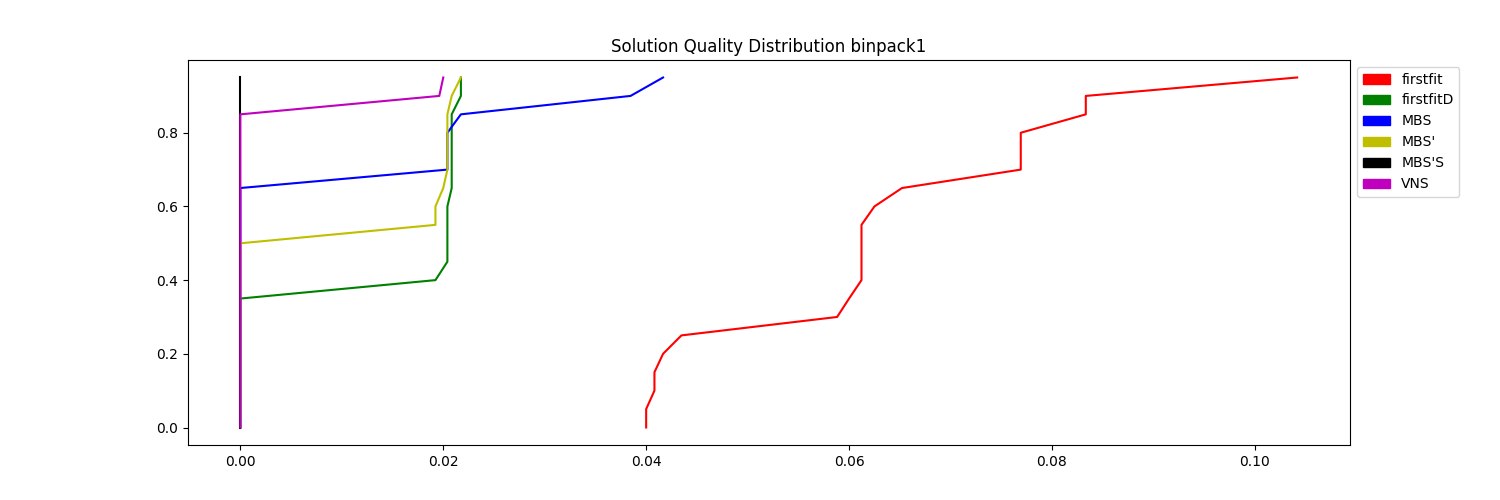
\includegraphics[scale=0.23]{pic/binpack1}
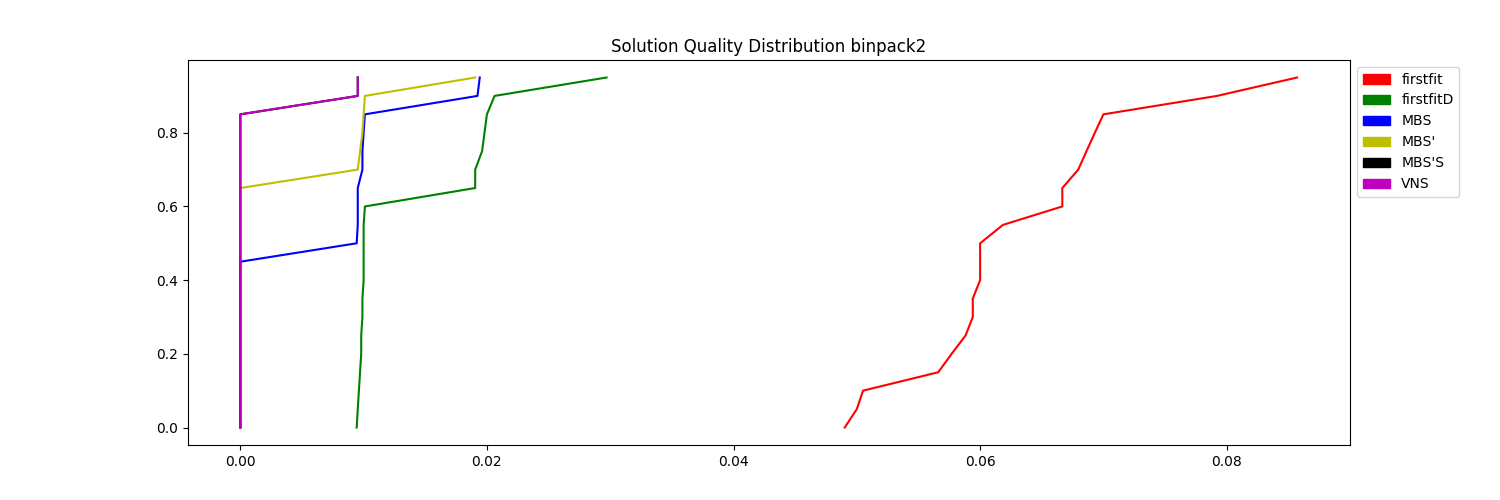
\includegraphics[scale=0.23]{pic/binpack2}

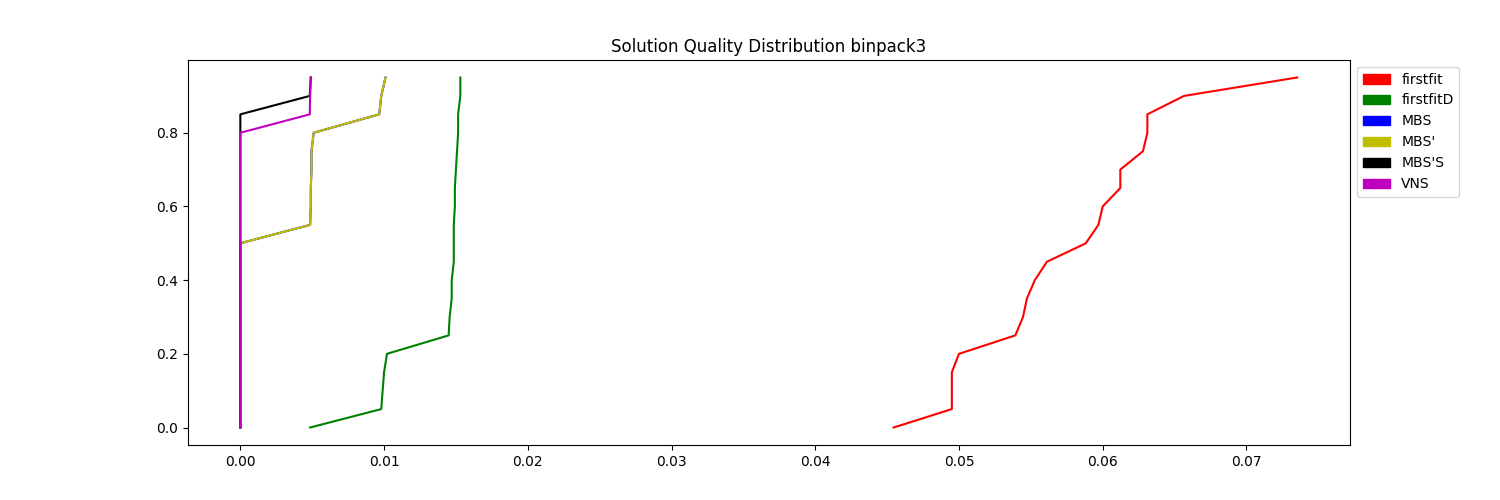
\includegraphics[scale=0.23]{pic/binpack3}
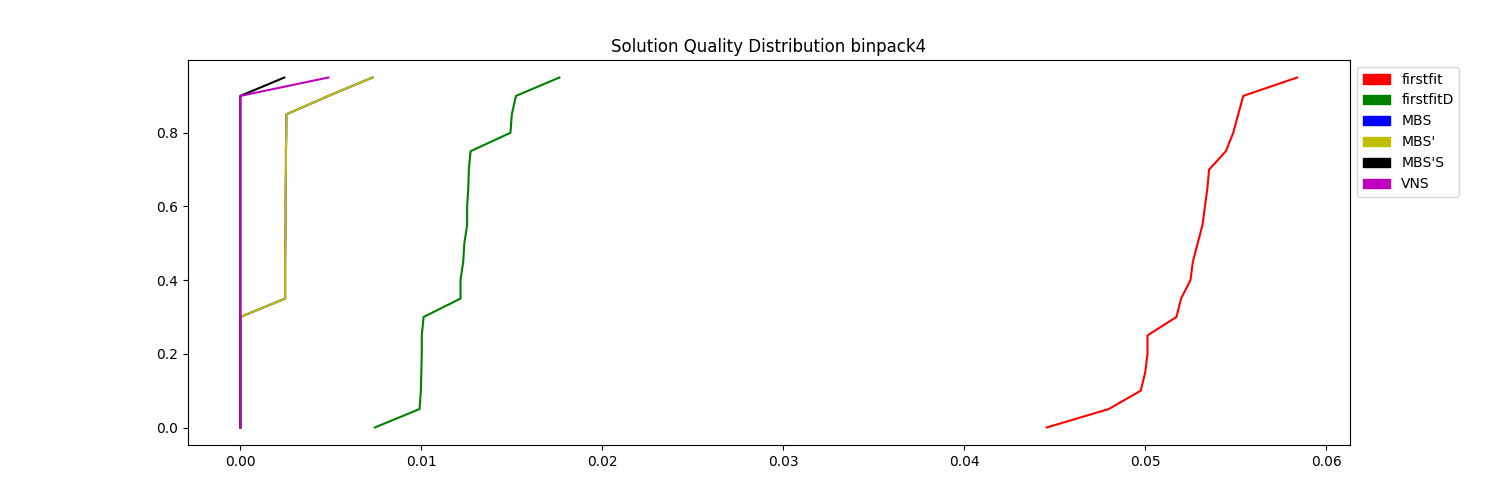
\includegraphics[scale=0.23]{pic/binpack4}
\caption{La prima classe del dataset.}
\end{table}

Per la seconda classe di problemi (Tabella 10), gli algoritmi si differenziano in maniera più netta.
\begin{table}[H]
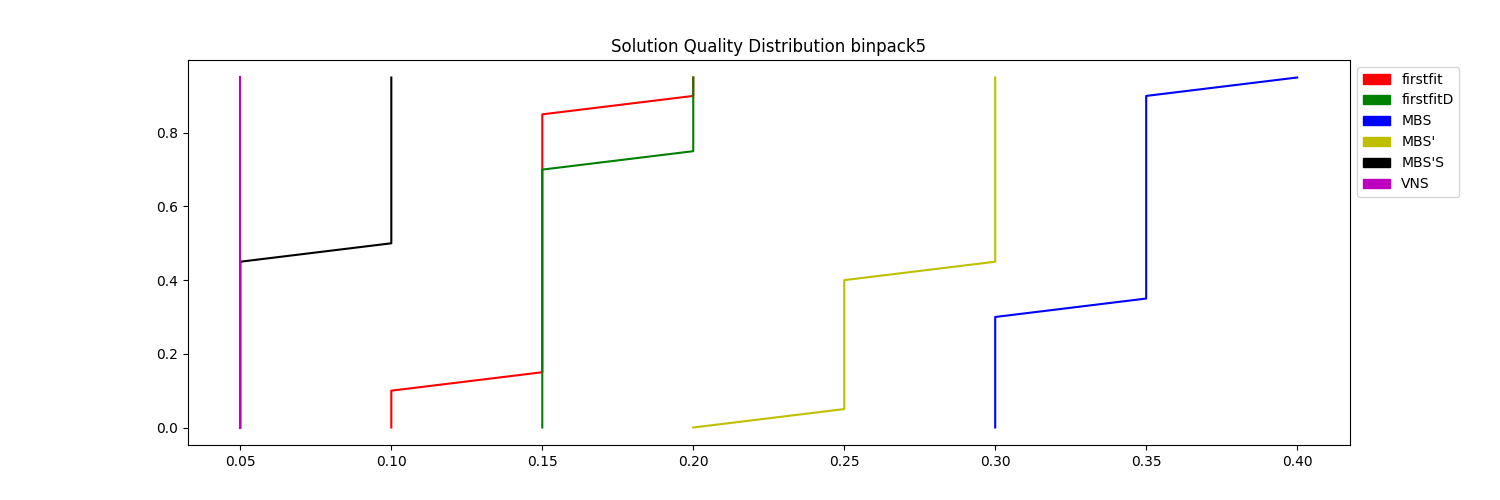
\includegraphics[scale=0.23]{pic/binpack5}
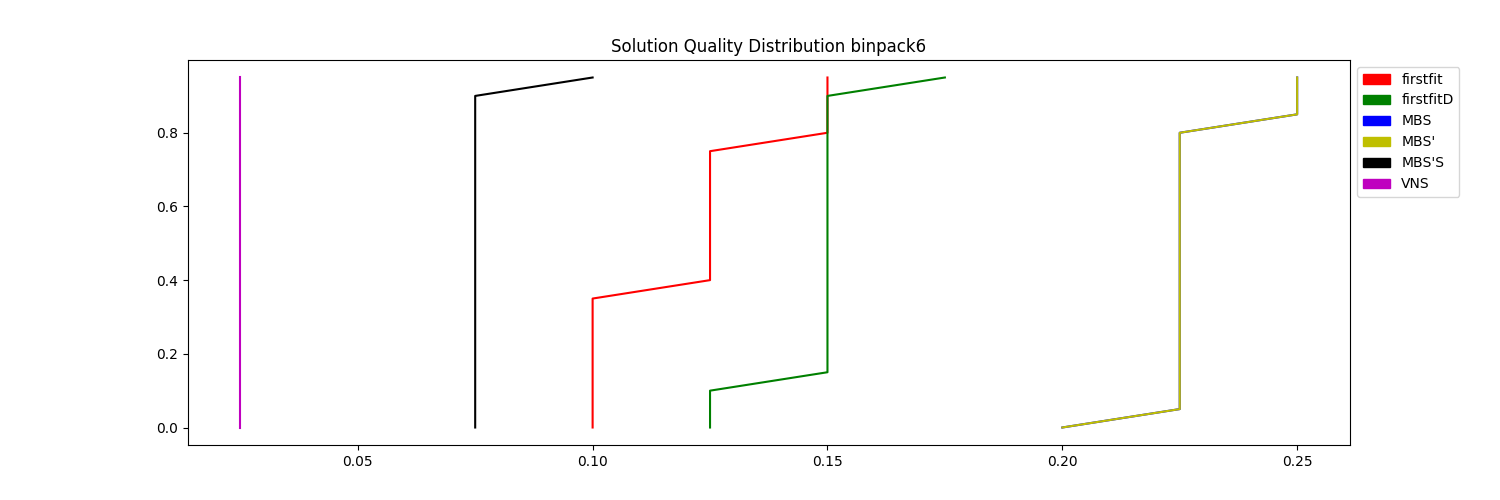
\includegraphics[scale=0.23]{pic/binpack6}

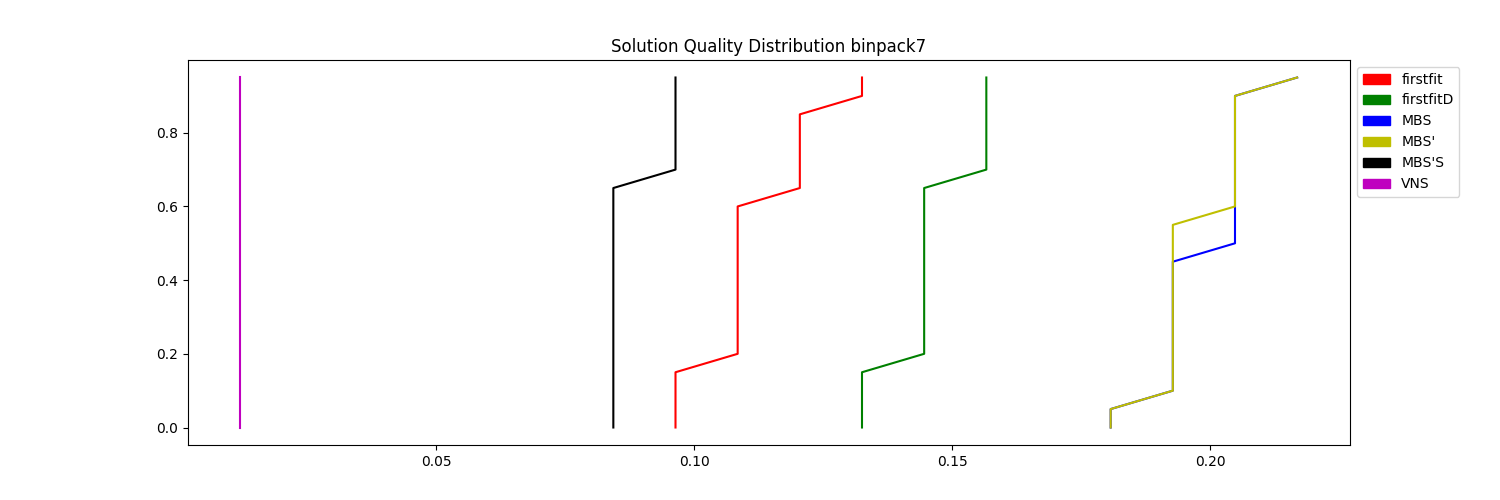
\includegraphics[scale=0.23]{pic/binpack7}
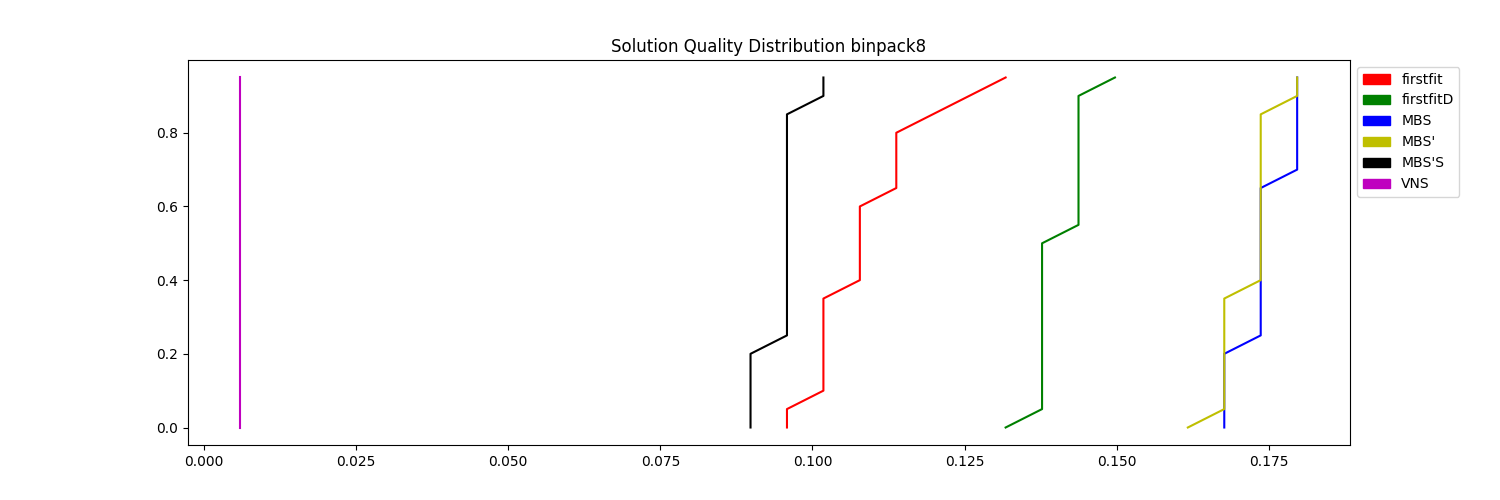
\includegraphics[scale=0.23]{pic/binpack8}
\caption{La seconda classe del dataset.}
\end{table}
\section{Lavori futuri}
Tra i possibili lavori futuri, oltre all'espansione del dataset di test e all'utilizzo di altre metriche di valutazione, tra cui quelle temporali, si propongono
\begin{itemize}
\item variazioni dei parametri delle metaeuristiche MBS sampling e VNS, con relativo confronto.
\item un possibile confronto diretto delle meta euristiche MBS sampling e VNS, fissando diversi tempi di esecuzione dei due algoritmi, in maniera tale da generare soluzioni equamente comparabili.
\item test di Wilcoxon per stabilire se due algoritmi comparabili siano significativamente distinti a livello di performance.
\end{itemize}  
\newpage
%----------------------------------------------------------------------------------------
\begin{thebibliography}{9}

\bibitem{Falkenauer}
  E.Falkenauer,
  \textit {"A Hybrid Grouping Genetic Algorithm for Bin Packing"},
 Working paper CRIF Industrial Management and Automation, CP 106 - P4, 50
av. F.D.Roosevelt, B-1050 Brussels (1994)
\end{thebibliography}
\end{document}